\chapter{Results and Discussions}
\label{ch:results}
 
This chapter presents the results of various tests conducted to verify the correctness and performance of the reference model for the CV32E40S core. We will discuss the types of tests performed, the performance and size of the reference model, and compare our approach to existing solutions. We will also discuss formal verification and highlight the advantages and limitations of our reference model implementation.

\section{Tests}
\label{sec:res_tests}

Multiple directed and random tests were used to verify the correctness of the reference model. Among other things, the tests cover the following complicated scenarios: 
\begin{itemize}
    \item Interrupt during different memory operations.
    \item Interrupt during multi-cycle instructions.
    \item Interrupt During CSR operations.
    \item Multiple simultaneous pending interrupts.
    \item Nested interrupts.
    \item Interrupts and exceptions simultaneously.
    \item Interrupts and debug requests simultaneously.
    \item Interrupts and \rv{wfi} instructions.
    \item Random instructions
    \item interrupt handler that goes straight to \rv{mret} (This is complicated because of the short time interrupts are disabled and re-enabled).
    \item CSR write to \rv{mie} that enables an interrupt to be taken.
    \item CSR write to \rv{mstatus} during interupts.
    \item New interrupt while the pipeline is flushing to take another interrupt.
\end{itemize}

The tests were run using core-v-verif run with Questasim 2021.4.2. 


For the purposes of our implementation, we assume the CV32E40S core operates correctly and verify our reference model against the CV32E40S version with the following git commit hash: \texttt{04947655f5642821f78904f8feb13dd677fbcc6d} \cite{openhwgroupCv32e40s2024}.
While we assume the CV32E40S is thoroughly verified and can be considered a golden model for our purposes, it might still contain undiscovered bugs. This presents a fundamental challenge in verifying the functionality of the reference model, as discrepancies between the two could be caused either by the core or by the reference model. This problem is exacerbated when configuring the reference model for a new processor core. In this case, neither the core nor reference model can be considered correct, and we can not verify the reference model against anything. When modifying the reference model for a new core, it is important to have a detailed specification of the intended design that the reference model can be modeled after.

Despite this, we still verify against the CV32E40S core, treating it as a golden model, as it can still indicate how the reference model behaves in various scenarios.


For the tests that pass, all instructions in the test report the same RVFI results in both the core and the reference model, while the failed tests have at least one mismatch. The results of these tests are shown in \Cref{tab:results}. For the failed tests, we list the faults below:
%The faults referred to in \Cref{tab:results} are listed below:
\begin{enumerate}[label=Fault \arabic*]
    \item An \rv{mret} instruction immediately following a \rv{dret} fails because the timing of \rv{prvl_lvl} is incorrect, causing a new interrupt to not be taken. \label{fault:mretdret}
    \item Incorrect state reversion after a debug request causes the wrong PC to be stored to \sv{depc}, and the reference model starts running the wrong instruction after the debug handler.\label{fault:revert}
    \item A write to \rv{mstatus} causes an interrupt not to be taken by the core but to be taken in the reference model. \label{fault:mstatus_write}
    \item A \rv{wfi} instruction is used at the end of some tests to stop the execution. The choice in \Cref{sec:wfi} causes Spike to ignore the \rv{wfi} and continue executing instructions after the end of the test program. \label{fault:wfi}
    \item\label{fault:trap} Spike causes \textit{Load address misaligned} trap not caused in the core.
    \item\label{fault:revert_csr} When storing the previous states in the ISS, the changes to the CSRs are not properly stored, causing changes to CSRs not to be properly reverted.
\end{enumerate}


\begin{table}
\centering
\caption{Table showing the results of multiple directed and random tests with the reference model.}
\label{tab:results}
\begin{tabular}{|l|c|c|}
\hline
\textbf{Test Name}                  & \textbf{Result}             & \textbf{Fault} \\
\hline
corev\_rand\_arithmetic\_base\_test & \cellcolor{green!25}Passed  &  \\
\hline
corev\_rand\_debug                  & \cellcolor{red!25}Failed    &  \ref{fault:wfi} \\
\hline
corev\_rand\_debug                  & \cellcolor{red!25}Failed    &  \ref{fault:wfi}\\
\hline
corev\_rand\_instr\_test            & \cellcolor{green!25}Passed  & \\
\hline
corev\_rand\_interrupt              & \cellcolor{green!25}Passed  & \\
\hline
corev\_rand\_interrupt              & \cellcolor{green!25}Passed  & \\
\hline
corev\_rand\_interrupt\_debug       & \cellcolor{red!25}Failed    &  \ref{fault:revert}\\
\hline
corev\_rand\_interrupt\_debug       & \cellcolor{red!25}Failed    &  \ref{fault:mretdret}\\
\hline
corev\_rand\_interrupt\_exception   & \cellcolor{red!25}Failed    &  \ref{fault:trap} \\
\hline
corev\_rand\_interrupt\_nested      & \cellcolor{red!25}Failed    &  \ref{fault:mstatus_write}\\
\hline
corev\_rand\_interrupt\_wfi         & \cellcolor{green!25}Passed  & \\
\hline
corev\_rand\_jump\_stress\_test     & \cellcolor{green!25}Passed  & \\
\hline
corev\_rand\_jump\_stress\_test     & \cellcolor{green!25}Passed  & \\
\hline
csr\_instructions                   & \cellcolor{green!25}Passed  & \\
\hline
custom\_interrupt\_test             & \cellcolor{green!25}Passed  & \\
\hline
debug\_test2                        & \cellcolor{red!25}Failed    &  \ref{fault:trap}\\
\hline
hello-world                         & \cellcolor{green!25}Passed  & \\
\hline
illegal                             & \cellcolor{green!25}Passed  & \\
\hline
riscv\_arithmetic\_basic\_test\_0   & \cellcolor{green!25}Passed  & \\
\hline
\end{tabular}
\end{table}


Despite these faults, the reference model successfully passed many tests, demonstrating its ability to handle complex scenarios involving interrupts and debug requests in many different scenarios. The individual identified faults might be relatively easy to fix, but the number of faults indicates that the complexity of the design has the potential to cause bugs. When modeling the reference model for a new core, bugs like these in the reference model might not be easy to find if the core is not yet implemented and compared to a faulty reference model.


%This problem arises because spike runs ahead of the core and the way \rv{mstatus.mie} is output from spike to properly time interrupts. When the first interrupt handler returns with \rv{mret}, setting \rv{mstatus.mie} high. When this change leaves WB in the pipeline shell, it allows spike to take the next interrupt, flush the pipeline, and fill up the pipeline. Because the second \rv{mret} happens so fast, the \rv{mstatus.mie = 0} change does not have time to go through the pipeline, so when the second \rv{mret} is run in spike, \rv{mstatus.mie} is still high and spike will take the next interrupt. All of this happens between two retirements in the core, so the RM will report the second interrupt instead of the first over RVFI.

\pagebreak

\section{Speed and size}
\label{sec:res_sizespeed}

\begin{sloppy}
We use the \lstinline{simstats} command to find the memory usage and simulation runtime with and without the reference model while running the random interrupt test. The memory usage is shown in \Cref{fig:res_size}, and the runtime is shown in \mbox{\Cref{fig:res_runtime}}. The size difference does not account for the size of Spike, so the $7\%$ increase in memory usage is likely because of the pipeline shell and surrounding components. The simulation runtime does, however, take into account the time used by Spike, and we see a $33\%$ increase in runtime with the reference model.
\end{sloppy}


\begin{figure}
\centering
\begin{minipage}{.43\textwidth}
    \resizebox{0.9\textwidth}{!}{%
    \centering
    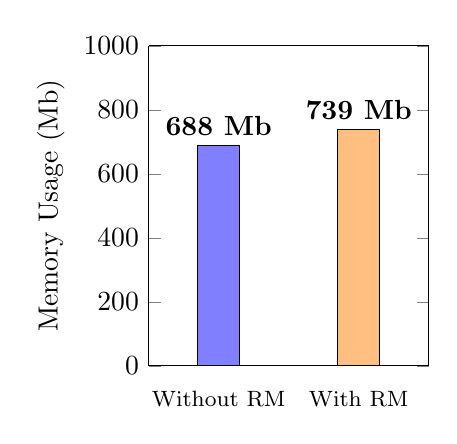
\begin{tikzpicture}
        \begin{axis}[
            /pgf/number format/1000 sep={},
            height=1.6in,   % Slightly increased height
            width=1.4in,   % Slightly increased height
            scale only axis,
            clip=false,
            separate axis lines,
            axis on top,
            xmin=0,
            xmax=4,
            xtick={1,3},
            x tick style={draw=none},
            xticklabels={},  % Removed default labels
            ymin=0,
            ymax=1000,
            ylabel={Memory Usage (Mb)},
            every axis plot/.append style={
                ybar,
                bar width=.6,
                bar shift=0pt,
                fill
            }
        ]
        \addplot[fill=blue!50] coordinates {(1,688)} node[above] {\textbf{688 Mb}};  % Custom label
        \addplot[fill=orange!50]  coordinates {(3,739)} node[above] {\textbf{739 Mb}};  % Custom label

        % Adding x-axis labels manually for better positioning
        \node[below, font=\footnotesize] at (axis cs: 1, -50) {Without RM}; 
        \node[below, font=\footnotesize] at (axis cs: 3, -50) {With RM};    
    \end{axis}
\end{tikzpicture}
}
\caption{Comarison of the memory usage of the simulation with and without a reference model.}
\label{fig:res_size}
\end{minipage}%
\begin{minipage}{.43\textwidth}
    \resizebox{0.9\textwidth}{!}{%
    \centering
    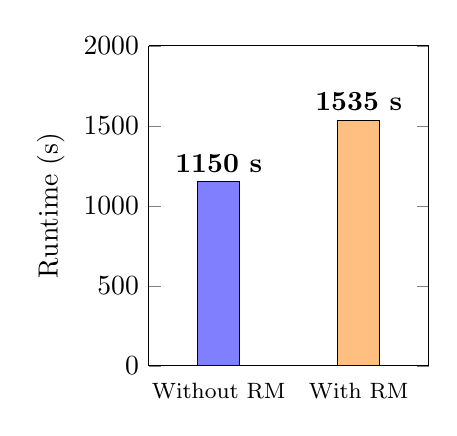
\begin{tikzpicture}[x=1mm, y=1mm]
        \begin{axis}[
            /pgf/number format/1000 sep={},
            height=1.6in,   % Slightly increased height
            width=1.4in,   % Slightly increased height
            scale only axis,
            clip=false,
            separate axis lines,
            axis on top,
            xmin=0,
            xmax=4,
            xtick={1,3},
            x tick style={draw=none},
            xticklabels={},  % Removed default labels
            ymin=0,
            ymax=2000,
            ylabel={Runtime (s)},
            every axis plot/.append style={
                ybar,
                bar width=.6,
                bar shift=0pt,
                fill
            }
        ]
        \addplot[fill=blue!50] coordinates {(1,1150)} node[above] {\textbf{1150 s}};  % Custom label
        \addplot[fill=orange!50]  coordinates {(3,1535)} node[above] {\textbf{1535 s}};  % Custom label

        % Adding x-axis labels manually for better positioning
        \node[below, font=\footnotesize] at (axis cs: 1, -50) {Without RM}; 
        \node[below, font=\footnotesize] at (axis cs: 3, -50) {With RM};    
    \end{axis}
\end{tikzpicture}
}
\caption{Comparison of the runtime of the simulation with and without a reference model.}
\label{fig:res_runtime}
\end{minipage}
\label{fig:sizespeed_comp}
\caption{Comparison of memory and runtime with and without a reference model.}
\end{figure}



%\subsection{Without reference model}
%
%\begin{terminal}
%# Memory Statistics                         
%#     mem: size after elab (VSZ)                 563.59 Mb
%#     mem: size during sim (VSZ)                 687.95 Mb
%# Elaboration Time                          
%#    elab: wall time                               6.38 s
%#    elab: cpu time                                5.37 s
%# Simulation Time                           
%#     sim: wall time                            1157.08 s
%#     sim: cpu time                             1149.94 s
%# Total Time                                
%#   total: wall time                            1163.46 s
%#   total: cpu time                             1155.31 s
%\end{terminal}
%
%\subsection{With reference model}
%
%\begin{terminal}
%# Memory Statistics                         
%#     mem: size after elab (VSZ)                 639.82 Mb
%#     mem: size during sim (VSZ)                 739.04 Mb
%# Elaboration Time                          
%#    elab: wall time                               6.79 s
%#    elab: cpu time                                5.88 s
%# Simulation Time                           
%#     sim: wall time                            1539.02 s
%#     sim: cpu time                             1535.19 s
%# Total Time                                
%#   total: wall time                            1545.81 s
%#   total: cpu time                             1541.07 s
%
%\end{terminal}


%Custom interrupt test
%
%\begin{terminal}
%# Memory Statistics                         
%#     mem: size after elab (VSZ)                 554.50 Mb
%#     mem: size during sim (VSZ)                 694.91 Mb
%# Elaboration Time                          
%#    elab: wall time                               5.05 s
%#    elab: cpu time                                4.32 s
%# Simulation Time                           
%#     sim: wall time                              43.73 s
%#     sim: cpu time                               30.89 s
%# Tcl Command Time                          
%#     cmd: wall time                             281.78 s
%#     cmd: cpu time                                2.73 s
%# Total Time                                
%#   total: wall time                             330.56 s
%#   total: cpu time                               37.94 s
%# 
%
%
%
%# Memory Statistics                         
%#     mem: size after elab (VSZ)                 554.50 Mb
%#     mem: size during sim (VSZ)                 693.93 Mb
%# Elaboration Time                          
%#    elab: wall time                               5.42 s
%#    elab: cpu time                                4.61 s
%# Simulation Time                           
%#     sim: wall time                              40.28 s
%#     sim: cpu time                               28.94 s
%# Tcl Command Time                          
%#     cmd: wall time                             659.66 s
%#     cmd: cpu time                                1.55 s
%# Total Time                                
%#   total: wall time                             705.36 s
%#   total: cpu time                               35.10 s
%# 
%
%
%
%# Memory Statistics                         
%#     mem: size after elab (VSZ)                 819.86 Mb
%#     mem: size during sim (VSZ)                 832.24 Mb
%# Elaboration Time                          
%#    elab: wall time                               4.19 s
%#    elab: cpu time                                4.19 s
%# Simulation Time                           
%#     sim: wall time                              40.86 s
%#     sim: cpu time                               29.25 s
%# Tcl Command Time                          
%#     cmd: wall time                              44.66 s
%#     cmd: cpu time                                1.31 s
%# Total Time                                
%#   total: wall time                              89.71 s
%#   total: cpu time                               34.75 s
%# 
%
%
%
%# Memory Statistics                         
%#     mem: size after elab (VSZ)                 554.50 Mb
%#     mem: size during sim (VSZ)                 693.93 Mb
%# Elaboration Time                          
%#    elab: wall time                               5.88 s
%#    elab: cpu time                                5.09 s
%# Simulation Time                           
%#     sim: wall time                              40.87 s
%#     sim: cpu time                               28.85 s
%# Tcl Command Time                          
%#     cmd: wall time                              40.85 s
%#     cmd: cpu time                                1.55 s
%# Total Time                                
%#   total: wall time                              87.60 s
%#   total: cpu time                               35.49 s
%# 
%
%# Memory Statistics                         
%#     mem: size after elab (VSZ)                 554.57 Mb
%#     mem: size during sim (VSZ)                 693.93 Mb
%# Elaboration Time                          
%#    elab: wall time                               5.82 s
%#    elab: cpu time                                5.06 s
%# Simulation Time                           
%#     sim: wall time                              45.40 s
%#     sim: cpu time                               31.79 s
%# Tcl Command Time                          
%#     cmd: wall time                              35.17 s
%#     cmd: cpu time                                1.63 s
%# Total Time                                
%#   total: wall time                              86.39 s
%#   total: cpu time                               38.48 s
%# 
%
%\end{terminal}
%
%\subsection{With reference model}
%
%\begin{terminal}
%# Memory Statistics                         
%#     mem: size after elab (VSZ)                 629.95 Mb
%#     mem: size during sim (VSZ)                 745.04 Mb
%# Elaboration Time                          
%#    elab: wall time                               6.65 s
%#    elab: cpu time                                6.01 s
%# Simulation Time                           
%#     sim: wall time                              50.99 s
%#     sim: cpu time                               36.22 s
%# Tcl Command Time                          
%#     cmd: wall time                              19.10 s
%#     cmd: cpu time                                2.48 s
%# Total Time                                
%#   total: wall time                              76.74 s
%#   total: cpu time                               44.71 s
%# 
%
%
%# Memory Statistics                         
%#     mem: size after elab (VSZ)                 629.93 Mb
%#     mem: size during sim (VSZ)                 745.04 Mb
%# Elaboration Time                          
%#    elab: wall time                               6.75 s
%#    elab: cpu time                                6.00 s
%# Simulation Time                           
%#     sim: wall time                              51.38 s
%#     sim: cpu time                               39.05 s
%# Tcl Command Time                          
%#     cmd: wall time                              72.82 s
%#     cmd: cpu time                                2.24 s
%# Total Time                                
%#   total: wall time                             130.95 s
%#   total: cpu time                               47.29 s
%# 
%
%
%# Memory Statistics                         
%#     mem: size after elab (VSZ)                 629.94 Mb
%#     mem: size during sim (VSZ)                 745.04 Mb
%# Elaboration Time                          
%#    elab: wall time                               6.21 s
%#    elab: cpu time                                5.49 s
%# Simulation Time                           
%#     sim: wall time                              49.74 s
%#     sim: cpu time                               38.17 s
%# Tcl Command Time                          
%#     cmd: wall time                              32.89 s
%#     cmd: cpu time                                1.51 s
%# Total Time                                
%#   total: wall time                              88.84 s
%#   total: cpu time                               45.17 s
%# 
%
%# Memory Statistics                         
%#     mem: size after elab (VSZ)                 629.92 Mb
%#     mem: size during sim (VSZ)                 745.12 Mb
%# Elaboration Time                          
%#    elab: wall time                               6.12 s
%#    elab: cpu time                                5.38 s
%# Simulation Time                           
%#     sim: wall time                              50.00 s
%#     sim: cpu time                               38.44 s
%# Tcl Command Time                          
%#     cmd: wall time                             131.77 s
%#     cmd: cpu time                                2.35 s
%# Total Time                                
%#   total: wall time                             187.89 s
%#   total: cpu time                               46.17 s
%# 
%
%
%# Memory Statistics                         
%#     mem: size after elab (VSZ)                 629.96 Mb
%#     mem: size during sim (VSZ)                 745.12 Mb
%# Elaboration Time                          
%#    elab: wall time                               6.15 s
%#    elab: cpu time                                5.45 s
%# Simulation Time                           
%#     sim: wall time                              50.50 s
%#     sim: cpu time                               37.90 s
%# Tcl Command Time                          
%#     cmd: wall time                              22.00 s
%#     cmd: cpu time                                2.34 s
%# Total Time                                
%#   total: wall time                              78.65 s
%#   total: cpu time                               45.69 s
%# 
%
%
%\end{terminal}


\section{Comparison to Previous Solutions}
\label{sec:res_comparison}

An important result of this report is how this implementation compares to other available solutions. The implementation will, therefore, be compared to using a traditional ISS, to the ImperasDV Verification IP, and the previous two-layered cycle-accurate approaches from \Cref{sec:bg_cycle-accurate}. We would ideally have access to all of these implementations and compare these by running the same tests with all of them to discover how they perform against each other. However, this is not the case. ImperasDV is closed and proprietary, and the previous two-layered approaches are not openly available or implemented for RISC-V. Instead of a quantitative comparison, we will use a few illustrative examples to qualitatively compare how we imagine the implementations would compare to each other based on assumptions made about their functionality.  We will also divide our reference model into our current and "ideal" implementations. Our current implementation differs from our ideal implementation since it injects the \sv{interrupt_allowed} signal directly into the core, as explained in \Cref{sec:interrupt_allowed}.

\subsection{Illustrative Examples}

To better understand the differences between the proposed reference model and previous solutions, we will consider three illustrative examples:

\begin{enumerate}[label=\textbf{Example \arabic*}]
    \item An interrupt is asserted when there is an outstanding memory request and the pipeline can not be flushed. This is the same example as shown in \Cref{fig:lw_sw_pipeline} and \Cref{fig:lw_sw_pipeline}.
    \item The same scenario as Example 1, but the core has a bug where \sv{interrupt_allowed} allows an interrupt to be taken despite outstanding memory requests.
    \item The core has a bug where interrupts are prioritized over asynchronous debug requests. A situation occurs where both an asynchronous debug request and an interrupt are applied at the same time. 
\end{enumerate}

%\begin{terminal}
%# UVM_ERROR @ 30654.300 ns : rvfi_compare_sva.sv(73) reporter [RVFI_COMPARE_ASSERT] MISMATCH PC: 00006104 rvfi_rm.rd1_wdata=80 rvfi_core.rd1_wdata=1880
%# UVM_ERROR @ 31074.300 ns : rvfi_compare_sva.sv(73) reporter [RVFI_COMPARE_ASSERT] MISMATCH PC: 00006104 rvfi_rm.rd1_wdata=80 rvfi_core.rd1_wdata=1880
%# UVM_ERROR @ 31377.300 ns : rvfi_compare_sva.sv(60) reporter [RVFI_COMPARE_ASSERT] MISMATCH PC: 000002ea rvfi_rm.mode=00000000 rvfi_core.mode=00000003                                        
%# UVM_ERROR @ 31380.300 ns : rvfi_compare_sva.sv(60) reporter [RVFI_COMPARE_ASSERT] MISMATCH PC: 000002ec rvfi_rm.mode=00000000 rvfi_core.mode=00000003
%# UVM_ERROR @ 31383.300 ns : rvfi_compare_sva.sv(60) reporter [RVFI_COMPARE_ASSERT] MISMATCH PC: 000002f0 rvfi_rm.mode=00000000 rvfi_core.mode=00000003
%
%\end{terminal}

%\tmp{Bør jeg ha med test resultater fra min løsning her? Hvordan kan det evt. gjøres ryddig når output er masse terminallinjer og PASSED eller FAIL på slutten, med evt MISMATCH}

\subsection{Traditional ISS}

\textcite{taylorAdvancedRISCVVerification2023} describe two ISS implementations, where asynchronous events are applied directly into the ISS and where asynchronous events are applied using RVFI. The problems with these implementations are introduced in \Cref{sec:back_issProblem}.
Because of their instruction accurate timing model, they have problems with asynchronous events. We will compare these solutions to our reference model using the examples below.

%\tmp{Jeg har ikke faktisk kjørt disse testene for en tradisjonell ISS, men bare forklart hva som (sansynligvis) hadde skjedd. Bør jeg prioritere å modifisere spike så jeg faktisk kan kjøre disse testene, eller holder det med forklaringen jeg har av testene her? }

%\tmp{For de andre løsningene har jeg jo ikke tilgang på de, så får uansett ikke kjørt tester.}

\subsubsection{Example 1}

The outcome of Example 1 when applying asynchronous events directly into an ISS is shown in \Cref{fig:lw_example}. This shows that the interrupt is taken immediately in the ISS, while the core retires 4 more instructions before taking the interrupt.

For an ISS controlled by RVFI, this problem would appear to be solved because it follows the interrupt execution from the core. This works for Example 1, but the problem will be highlighted with Example 2 and 3.

This example is taken from \rv{custom_interrupt_test}, where we see that our reference model passes in \Cref{sec:res_tests}.

\subsubsection{Example 2}

In example 2, the same test is run, but the core has a bug where the interrupts are taken regardless of outstanding memory requests. This test highlights the problem with interrupts following the RVFI from the core in a traditional ISS. 
Looking at \Cref{fig:lw_sw_pipeline}, we imagine that the bug causes the interrupt to be taken instead of PC \rv{147c}. When the core incorrectly takes the interrupt and returns the result over RVFI, the ISS would also take the interrupt at the same instruction. This could leave the bug undetected.

For our current implementation that depends on \sv{interrupt_allowed} from the core, we would have the same problem. Since the bug is with the \sv{interrupt_allowed} signal, injecting the faulty signal from the core would lead to the same bug in our reference model. This is one of the largest disadvantages of our current implementation. 

If we instead look at our "ideal" solution where we model the \sv{interrupt_allowed} signal according to the state of the pipeline shell, this would give a better result. Assuming that the \sv{interrupt_allowed} signal in the reference model is properly recreated from a correct specification, the reference model would not allow an interrupt to be taken with outstanding memory requests, leading to a mismatch between the reference model and the core.


\subsubsection{Example 3}

In example 3, both a debug request and an interrupt are injected, and the core has a bug where the prioritization between these is wrong. 

Considering the ISS that follows RVFI, we believe this bug would not be found. Since the core reports taking an interrupt instead of correctly taking the debug request, the ISS will follow the RVFI output and also take the interrupt. As with example 2, this bug would also go unnoticed. 

Since the bug in the core is not related to \sv{interrupt_allowed} or \mbox{\sv{async_debug_allowed},} but with the actual prioritization, our implementation will find this bug and report a mismatch between the core and the reference model. Compared to the ISS solution, our implementation only uses \sv{interrupt_allowed} to determine if the interrupt is allowed, but it does not use it to decide between taking interrupts or debug requests.

%Using the Spike implementation used with the CVA6 core as an example, this uses \sv{write_rvfi_instruction()}, which takes in the rvfi output from the core and passes it to spike. 

%Using the step-and-compare 2.0 approach discussed in \cite{taylorAdvancedRISCVVerification2023} as an example, one approach to support asynchronous events is to only connect asynchronous events to the core and not the ISS. When the core reports that an interrupt or debug request is taken over \acrshort{rvfi}, this is passed to the ISS, which then also takes the specified interrupt or debug request. The problem with this approach is that it is not able to correctly verify which asynchronous event should be taken and if this is taken at the correct instruction. 
%
%The implementation discussed in this report attempts to solve this problem. Our reference model takes asynchronous interrutps and debug requests as inputs to the model and uses these independently of the core to determine how the processor should respond to the various inputs. 
%
%Our current implementation does rely on the \sv{interrupt_allowed} signal from the core to determine if an interrupt is allowed to be taken. Although it does depend on the core, the reference model still independently decides which interrupt or debug request should be taken, minimizing the verification hole present in a traditional ISS.


Our current implementation has a smaller verification gap than a traditional ISS, even when directly injecting \sv{interrupt_allowed} from the core. If this signal is generated completely from the pipeline shell, we would have a smaller verification gap.


\subsection{ImperasDV}

Since ImperasDV is proprietary, we can not exactly know how it works. The following discussion and comparison are based on assumptions about its functionality based on surrounding modules and output logs, but we can not be certain about its operation. The assumed behavior of ImperasDV is introduced in \Cref{sec:imperasdv}. We assume it handles asynchronous events by forking the execution to explore possible state changes. 
ImperasDV analyzes the possible next states, considering the next instruction and incoming asynchronous events. It then goes down each fork to see if it ends up in the same state as the DUT.

%ImperasDV is used with \acrshort{rvvi}, where CSRs and memory regions modified asynchronously are marked as volatile. Asyncronous inputs to the core like \sv{irq} and \sv{haltreq} are passed to ImperasDV as net changes. 


The problem (and advantage) of this is that it does not contain core-specific pipeline details but executes every possible next state. If the core, for example, took an interrupt that should not have been taken because of pipeline details, this could possibly not be detected. 

\subsubsection{Example 1}


Using the example from \Cref{fig:lw_sw_pipeline}, where an interrupt is asserted when interrupts are not allowed, we assume the following functionality in ImperasDV.

ImperasDV would have a fork with two possible states for each instruction after the interrupt is asserted. It could either retire the next instruction or take the interrupt. For each retirement, it would attempt both and check if any of the results match the results from the core. In our example, it would see that retiring \rv{147a},\rv{147c}, and \rv{147e} match with the core. When deciding between retiring \rv{1480} and taking the interrupt, it decides that taking the interrupt matches the execution of the core.

This way, it determines that the interrupt is one of the legal states, but without proper pipeline information, we believe that it can not verify if taking the interrupt at that point was legal.

\subsubsection{Example 2}

Evaluating example 2, with a bug in \sv{interrupt_allowed}, we assume the following behavior. 

We assume ImperasDV uses a similar fork from example 1, where for every retirement, it attempts both taking the interrupt or retiring the next instruction and evaluates what matches. 

The bug could make the core take the interrupt after retiring \rv{147c}. Since this was one of the possible states in ImperasDV, it would not mark this as a mistake and continue execution.

We see that ImperasDV can allow a superset of the actual allowed states, which can leave bugs undetected.

This is similar to the behavior of our current solution that relies on \sv{interrupt_allowed} from the core, which does not detect this bug either and performs the same as ImperasDV. 
However, when considering our ideal solution, we believe it would detect the bug, outperforming ImperasDV in this example.

%Looking at our solution, we will differentiate between our actual implemented solution which relies on the \sv{interrupt_allowed} signal from the core, and our proposed solution, where \sv{interrupt_allowed} is generated by the pipeline shell.

%In our implemented solution, bugs in the core that influences the \sv{interrupt_allowed} signal also influences the execution of the core. Looking at the same example as ImperasDV in \Cref{fig:lw_sw_pipeline}, since the bug would change the \sv{interrupt_allowed} signal, our solution would also function the same way as the core, taking the interrupt at the incorrect time.

%However, if the \sv{interrupt_allowed} signal is recreated based on information in the pipeline shell, the interrupt would be taken at different times in the core and reference model, and the bug would be found.

\subsubsection{Example 3}

Evaluating Example 3, where an asynchronous debug request and an interrupt are applied simultaneously, and the core has a bug prioritizing interrupts over debug requests, we expect the following behavior.

When the interrupt and debug request are asserted, ImperasDV forks its execution and attempts: a) retiring the next instruction, b) taking the debug request, and c) taking the interrupt. It discovers that taking the interrupt matches the execution of the core. Here, we believe the bug is not detected since both taking the interrupt and debug request were possible state changes in ImperasDV. 

\begin{sloppy}
In our current implementation, which relies on \sv{interrupt_allowed}, the core only decides if interrupts are allowed. Our implementation can independently decide if an interrupt or debug should be taken, even though it relies on \mbox{\sv{interrupt_allowed}}. In this situation, our current and ideal solution would find the bug, while we assume that ImperasDV would not. 
\end{sloppy}

\subsection{Previous Two-Layered approaches}

Our implementation has many similarities to the two-layered approaches from \textcite{leeFaCSimFastCycleAccurate2008} and \textcite{chiangEfficientTwolayeredCycleaccurate2009} introduced in \Cref{sec:bg_cycle-accurate}. As with our implementation, they feature one functional, untimed kernel and one timing shell responsible for the correct cycle-accurate timing of the results from the functional kernel. 

The major difference between these and our solution is in the design of the timing shell. \textcite{chiangEfficientTwolayeredCycleaccurate2009} solution uses a scheduler that distributes the state changes into different cycle slots, as shown in \Cref{fig:timeshell}. 
\textcite{leeFaCSimFastCycleAccurate2008} instead computes the number of elapsed cycles for each pipeline stage as a chunk, and uses this to advance the core clock, instead of simulating the pipeline cycle-by-cycle.

We instead use use pipeline slots to simulate the movement of instructions through the pipeline, where a controller module decides at which cycles the instructions should step through the pipeline. This more closely relates to an actual pipeline implementation, making the functionality easier to understand and implement.

Neither of the previous two-layered implementations is publicly available or implemented for RISC-V, and none of the solutions specify how they would work in lock-step execution.
FaCSim is meant to be used for performance evaluation and architectural exploration \cite{leeFaCSimFastCycleAccurate2008}. It claims to have an error margin of $6.79 \%$, compared to the $100 \%$ cycle-accurate simulator, ARMulator \cite{leeFaCSimFastCycleAccurate2008}.

For a cycle-accurate simulator to be used for verification, we would ideally have 0 errors. A randomly generated core-v-verif test usually contains 5000 to 50000 instructions \cite{openhwgroupOpenhwgroupCorevverif2023}. With an error margin of $7 \%$, the implementation would lead to many mismatches if used directly as a cycle-accurate simulator running parallel to the core. 


%Another difference One difference is that Chiang and Huangs timing shell is implemented in SystemC, while our pipeline shell is implemented in SystemVerilog. This allows for the ISS to be replaced with a SystemVerilog compiled ISS in the future, in order to support formal verification.  


Although a fully cycle-accurate comparison between the core and reference model is hard to achieve with this implementation, the important aspect is that instructions are ordered correctly at the instruction level (\Cref{rmReq:order}. This does not necessarily require full cycle accuracy if lock-step execution is implemented with this solution. By waiting until both the core and reference model have retired before comparing the two, we might mitigate some of these errors. However, inaccuracies mean we cannot fully trust the results.

Since both these previous implementations also rely on core-specific functionality and influenced the design of our reference model, we assume that they would perform similarly to the implementation proposed in this thesis for the examples above.
Because of this, and because we do not know the details of the implementation, we will not compare each of the examples in detail, as we did for the previous solutions.
We assume they would depend on pipeline information similar to the reference model and be susceptible to the same potential bugs and inaccuracies as the reference model. However, as described in \Cref{sec:pw_pipelineShellDesign}, we believe the cycle-based approach could be more complex to model compared to our reference model design.


%Since a direct comparison of functionality is not possible, and the functionality is very . We will compare these to our implementation using the previous examples and assume how they would operate.



\section{Formal Verification}
\label{sec:res_formal}

Since we use the Spike ISS, which is incompatible with formal verification, our reference model is also incompatible with formal verification. However, the rest of the design is designed to support formal verification in the future with a "formal-friendly" ISS. Therefore, we want to test if the rest of the design is compatible with formal verification.

We test formal verification of the design at two points during the development of the reference model, with two different purposes.
The first test was during \Cref{phase:rvfi_interrupt} of the implementation strategy from \Cref{sec:strategy}, where we passed interrupts in sync with RVFI from the core into the ISS. At this point, the design resembled a traditional ISS implementation without a pipeline shell. During this phase, we implemented the initial formal verification support and RVFI comparison assertions. Because the pipeline shell was not yet implemented, using a dummy ISS as explained in \Cref{sec:formal_dummy}, we could test that all the assertions in the comparison module worked correctly and that the design and processor core loaded correctly into Onespin. 

The second formal verification test is at the end of the development, with an implemented pipeline shell in \Cref{phase:pipeline_shell}. Using a simple dummy ISS, we can not verify the correctness of the pipeline shell since this requires a working ISS, but we can verify that the pipeline shell is synthesizable and can compile in Onespin. Because of the introduced timing differences caused by the pipeline shell, the assertions from the previous phase no longer work, but we see that the pipeline shell design can run in Onespin

Using both these tests, in conjunction with the functional tests using simulation-based verification, we can assume that the pipeline shell can work with formal verification in Onespin. This requires that the ISS is replaced with a synthesizable ISS compatible with the interface described in this thesis.